\documentclass[border=3pt]{standalone}
\usepackage{tikz}
\usetikzlibrary{arrows.meta,calc,positioning}
\tikzset{pin/.style={-{Stealth[length=5pt]}},
  blk/.style={draw, thick, font=\sffamily\small, align=center}}
\begin{document}
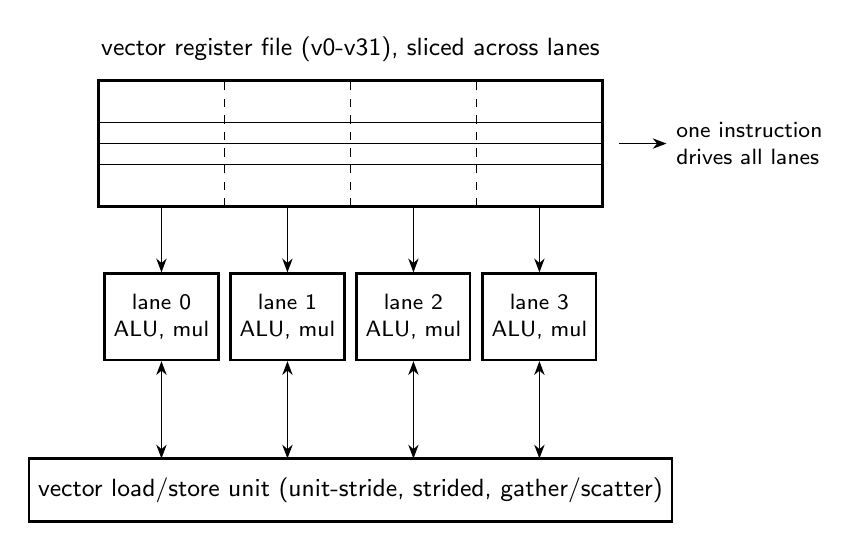
\begin{tikzpicture}[font=\sffamily\small]
  % vector register file (sliced across lanes)
  \node[blk, minimum width=64mm, minimum height=16mm] (vrf) at (0,0) {};
  \node[font=\sffamily\small, above=1mm of vrf.north] {vector register file (v0-v31), sliced across lanes};
  \foreach \x in {-1.6,0,1.6}{\draw[dashed] (\x,-0.8) -- (\x,0.8);}
  \foreach \y in {-2.7,0,2.7}{\draw ($(vrf.west)+(0,\y mm)$) -- ($(vrf.east)+(0,\y mm)$);}
  % lanes
  \foreach \i/\x in {0/-2.4, 1/-0.8, 2/0.8, 3/2.4}{
    \node[blk, minimum width=14mm, minimum height=11mm, font=\sffamily\footnotesize] (l\i) at (\x,-2.2) {lane \i\\ALU, mul};
    \draw[pin] (\x,-0.8) -- (l\i.north);
  }
  % memory unit
  \node[blk, minimum width=40mm, minimum height=8mm] (mem) at (0,-4.4) {vector load/store unit (unit-stride, strided, gather/scatter)};
  \foreach \i/\x in {0/-2.4, 1/-0.8, 2/0.8, 3/2.4}{
    \draw[{Stealth[length=5pt]}-{Stealth[length=5pt]}] (l\i.south) -- (\x,-4.0);}
  \draw[pin] ($(vrf.east)+(2mm,0)$) -- ++(6mm,0) node[right, align=left, font=\sffamily\footnotesize]{one instruction\\drives all lanes};
\end{tikzpicture}
\end{document}
